\RequirePackage[2020-02-02]{latexrelease}
\documentclass[manuscript]{clv3}
%\documentclass[final]{clv3} % use  for the final version

\usepackage{hyperref}
\usepackage{xcolor}
\definecolor{darkblue}{rgb}{0, 0, 0.5}
\hypersetup{colorlinks=true,citecolor=darkblue, linkcolor=darkblue, urlcolor=darkblue}

\bibliographystyle{compling}

% test compatibility with algorithmic.sty
%\usepackage{algorithmic}

%\thispagestyle{plain}
\pagenumbering{gobble}
    \begin{center}
    
        \vspace*{1cm}

        \large
        \textcolor{darkblue}{Faculty of Arts}
        
        \vspace{0.5cm}
        Master’s Thesis 
        
        \vspace{0.5cm}
        Digital Text Analysis 
        
       \vspace{1.5cm}
            
        \Huge
        \textcolor{darkblue}{\textbf{A GPT-Powered Approach 
to Data Augmentation for 
Multi-Label Emotion 
Classification}}
            
        \vspace{0.5cm}
        \LARGE
        \textcolor{darkblue}{}
            
        \vspace{1.5cm}
        
        \Large    
        \textcolor{darkblue}{Marija Kliocaite}
        
        \vspace{0.5cm}
        
        \large
        \textcolor{darkblue}{Supervisor: Prof. Dr. Walter Daelemans}
        
        \vspace{0.5cm}
        \textcolor{darkblue}{Co-supervisor: Jens Van Nooten}
        
        \vspace{0.5cm}
        \textcolor{darkblue}{Assessor: Simon Blanchard}
        
        %\vfill
        \vspace{1cm}
        \textcolor{darkblue}{University of Antwerp}
        
        \vspace{1cm}   
        \textcolor{darkblue}{Academic year 2023–2024}
            
    \end{center}

\issue{1}{1}{2016}

%Document Head
%\dochead{A GPT-powered approach to data
%augmentation and multi-label
%emotion classification!}

\runningtitle{A GPT-Powered Approach to DA for ML
Emotion Classification}

\runningauthor{Marija Kliocaite}

\begin{document}

\thispagestyle{plain}
\pagenumbering{gobble}
    \begin{center}
    
        \vspace*{1cm}

        \large
        \textcolor{darkblue}{Faculty of Arts}
        
        \vspace{0.5cm}
        Master’s Thesis 
        
        \vspace{0.5cm}
        Digital Text Analysis 
        
       \vspace{1.5cm}
            
        \Huge
        \textcolor{darkblue}{\textbf{A GPT-Powered Approach 
to Data Augmentation for 
Multi-Label Emotion 
Classification}}
            
        \vspace{0.5cm}
        \LARGE
        \textcolor{darkblue}{}
            
        \vspace{1.5cm}
        
        \Large    
        \textcolor{darkblue}{Marija Kliocaite}
        
        \vspace{0.5cm}
        
        \large
        \textcolor{darkblue}{Supervisor: Prof. Dr. Walter Daelemans}
        
        \vspace{0.5cm}
        \textcolor{darkblue}{Co-supervisor: Jens Van Nooten}
        
        \vspace{0.5cm}
        \textcolor{darkblue}{Assessor: Simon Blanchard}
        
        %\vfill
        \vspace{1cm}
        \textcolor{darkblue}{University of Antwerp}
        
        \vspace{1cm}   
        \textcolor{darkblue}{Academic year 2023–2024}
            
    \end{center} % !!!!
\clearpage
\thispagestyle{plain}
\pagenumbering{gobble}
\begin{center}

The undersigned, Marija Kliocaite, student of the Master program in Digital Text Analysis at the University of Antwerp, declares that this thesis is completely original and exclusively written by herself / himself. For all information and ideas derived from other sources, the undersigned has referred to the original sources, both explicitly and in detail.
 
\end{center}
 % !!!!
\let\cleardoublepage\clearpage


\title{A GPT-Powered Approach to Data
Augmentation for Multi-Label
Emotion Classification}

\author{Marija Kliocaite}

\maketitle

\pagenumbering{arabic} % !!!

\begin{abstract}
This article investigates the application of Large Language Models (LLMs) for improving multi-label classification accuracy with LLM-augmented data. Specifically, we employ the GPT-4o-mini model to generate synthetic instances for the emotion classification of the SemEval-2018 Task 1: Affect in tweets dataset, demonstrating the potential of LLMs to address data scarcity challenges in multi-label scenarios. In order to classify both the augmented and original data into multiple emotions, we employ BERT and RoBERTa models. We experiment with prompting GPT-4o-mini to adopt different personality traits based on the OCEAN model to assess the impact on data generation quality. In addition, we examine how representative the generated data for emotion labels is through calculating data typicality and type-token ratio. While the incorporation of GPT-generated data demonstrated efficacy in addressing class imbalance, the inclusion of personality traits through role-based prompting yielded minimal impact on data diversity and model performance.

Keywords: multi-label emotion classification, data augmentation, class imbalance, language models, GPT-4o, social media
\end{abstract}

\section{Introduction}

In fields such as healthcare, finance, and marketing, the ability to recognize and interpret complex data patterns is crucial for making informed decisions and staying competitive. For many businesses and organizations, this capability is essential for strategic advantage. Consequently, machine learning models have emerged as valuable tools for addressing these complex pattern recognition challenges. Nevertheless, data gathering is often the hardest and the slowest part of machine learning projects. This raises the question of effectiveness and cost-efficiency of building such models.

Further complicating the data gathering process, Natural Language Processing (NLP) introduces additional challenges specific to text classification due to the inherent ambiguity of human language. Unlike structured data, text data often exhibits vagueness and subjectivity, making it challenging to categorize with high accuracy. A prime example of frequently encountered challenges is the common co-occurrence of multiple emotions within a single text, posing further difficulties in the training and evaluation processes. Moreover, the task of assigning multiple labels to a text, known as multi-label text classification, is further complicated by class imbalance, where certain categories are over-represented compared to others \cite{li-etal-2023-enhancing-extreme}. This paper addresses these challenges by exploring novel approaches to data augmentation. 

With the recent surge in computational power, LLMs have emerged as powerful tools, prompting researchers to explore their vast potential. Addressing the challenge of class imbalance in emotion recognition, researchers are actively exploring the potential offered by various LLM architectures, such as OpenAI's decoder-based GPT models, known for their generative capabilities and ability to create synthetic data. Additionally, researchers have explored variations of encoder-based language models (LMs), such as BERT or RoBERTa, for their ability to improve classification performance, particularly in imbalanced datasets \cite{DBLP:journals/corr/abs-2003-02245, 10.1145/3357384.3358040, 10.1145/3544548.3580688, yoo2021gpt3mix, van-nooten-daelemans-2023-improving, møller2023prompt, zhang2020data, li2023synthetic}. While the effectiveness of Data Augmentation (DA) through this approach may vary, the potential benefits are nonetheless promising \cite{10.1016/j.eswa.2022.118534}. In addition, LLMs offer the potential benefits of lower financial costs and increased efficiency in terms of time for data collection. On the other hand, the generated data might still exhibit stylistic rigidity. The guardrails imposed by Reinforcement Learning with Human Feedback (RLHF) can constrain the data to a limited set of statistical patterns, potentially hindering the model's ability to learn the full spectrum of language use, and thus produce more diverse and interesting data \cite{van-nooten-daelemans-2023-improving}.

This paper aims to leverage the capabilities of LLMs to address the challenge of class imbalance in multi-label text classification tasks. Specifically, it will investigate the abilities of OpenAI's GPT-4o-mini model and bidirectional transformers BERT and RoBERTa on tackling a multi-label problem. The OpenAI model will be employed to perform DA on an imbalanced dataset of tweets labeled with 11 emotions. Following the DA process, the augmented data will then be used to train and evaluate multi-label classification models through BERT and RoBERTa. The ultimate goal of the present study is multifold: first, the capabilities of LLMs as generators of qualitative synthetic data are compared with previously established DA methods. Second, several prompting strategies are explored to add more diversity to the generated data by incorporating a range of personalities through leveraging the OCEAN model's framework \cite{article}. Our hypothesis is that the inclusion of roles in prompts would lead to more diverse GPT-generated data. Third, the performance of LMs trained on the augmented data is compared with a number of baselines and previous state-of-the-art \cite{10.1016/j.eswa.2022.118534}. 
Building the foundation for this research, several key questions are posed:
\begin{enumerate}
    \item To what degree does the implementation of synthetic data augmentation contribute to enhancing the performance of models in handling a multi-label classification task?
    \item  Can we diversify generated synthetic data by assigning a personality type to an LLM?
    \item Can models effectively handle a multi-label classification problem characterized by class imbalance?
\end{enumerate}

The paper is structured in the following way: Section 2 provides a comprehensive overview of relevant work on multi-label classification and emotion recognition, including techniques for data augmentation. It also explores innovative use of LLMs for data augmentation and various prompting strategies for GPT models on eliciting emotional responses. Section 3 delves into the details of the dataset used in this paper, and describes the baseline models employed in the experiments. This section also discusses model evaluation metrics and the specific prompting strategy applied in this research. Section 4 presents the main results of the experiments and discusses the further implications of these findings. Finally, in Section 5, we draw key conclusions, acknowledge the limitations of the present work and propose avenues for further explorations on the subject.

\section{Related Work}
\subsection{Multi-label Emotion Recognition Task}
Within the research domain of text classification, multi-class problems involving single-label emotion identification, where the goal is to determine the primary emotion expressed within a text, have garnered a lot of attention. This is particularly evident when analyzing social media data, where understanding user sentiment and emotional states is crucial for various applications such as marketing, customer service, and public opinion analysis. However, accurately identifying multiple emotions within a single piece of text remains a challenge due to the complex interplay of emotional expressions, ambiguities in natural language, and the potential for overlapping or contradictory emotional cues. 

To address this issue, researchers have explored various solutions for multi-label emotion classification tasks. One prominent dataset used for model training is the \textit{GoEmotions} \cite{demszky-etal-2020-goemotions} dataset composed of Reddit comments and annotated for 27 emotions. As previously stated by \citet{demszky-etal-2020-goemotions}, the dataset has a range of applications, ranging from the development of empathetic chatbots to the detection of harmful online behavior. However, the main drawback of this dataset is the lack of multi-label examples, which limits its effectiveness in training models for complex scenarios where multiple emotions coexist.

As the \textit{GoEmotions} dataset presents a number of limitations, more suitable multi-label resources exist for our purposes. In particular, the \textit{SemEval} series of competitions significantly contributed to the advancements in the field. For instance, the \textit{SemEval-2018 Task-1: Affect in Tweets} attracted 57 participants tackling multi-label emotion classification across three languages: English, Arabic, and Spanish \cite{10.1016/j.eswa.2022.118534}. By the end of the competition, the solution of \citet{baziotis2018ntuaslp} established a new benchmark by setting the highest state-of-the-art results on this dataset. However, while the distribution of emotions in the dataset reflects a natural imbalance, there remains an issue of rarer classes having insufficient representation for the training of ML models.

Additionally, the difference in label distribution between the two datasets is evident from the average number of labels per entry: 1.17 for the \textit{GoEmotions} dataset and 2.34 for the \textit{SemEval} dataset. Thus, to push the boundaries of current multi-label emotion recognition models, we leverage the \textit{SemEval-2018 Task-1} dataset, which features tweets with richer annotations of co-occurring emotions. However, illustrating the imbalanced distribution, the emotions such as anger, disgust, joy, and sadness received significantly more annotations than neutral, surprise, and trust \cite{10.1016/j.eswa.2022.118534}. Nevertheless, the presence of multiple emotion labels within the tweets makes this dataset particularly well-suited for our investigation into multi-label emotion recognition. 

Several solutions have been proposed to address the problem presented by the previously described dataset. The state-of-the-art results, which were achieved by \citet{baziotis2018ntuaslp}, yielded a model with an accuracy of 58.8\% (multi-label accuracy, also known as Jaccard index), F1-micro of 70.1\% and F1-macro of 52.8\%. This performance was achieved using a Bi-LSTM architecture incorporating a multi-layer attention mechanism, featuring also word2vec embeddings trained on an extensive collection of English tweets. As for the hyperparameter tuning, the authors employed Bayesian optimization \cite{baziotis2018ntuaslp, 10.1016/j.eswa.2022.118534}, a method known for its efficiency in exploring high-dimensional spaces compared to traditional grid or random search approaches.

Subsequently, \citet{10.1016/j.eswa.2022.118534} have achieved an improvement on the results of \citet{baziotis2018ntuaslp}, reaching the accuracy of 62.4\% (3.6\% gain over the previous state-of-the-art score), F1-micro 74.2\% and F1-macro 60.3\%. In order to obtain these classification results, a RoBERTa-MA (RoBERTa Multi-Attention) model was used. In addition to this, the authors noted that certain labels,  such as "\textit{disgust}" and "\textit{optimism}", were more challenging to identify. These labels yielded the lowest class-specific accuracies of 79.4\% and 77.7\% respectively, compared to other classes. Interestingly, these labels are not underrepresented, in contrast to "\textit{surprise}" and "\textit{trust}" labels, which yielded higher class-specific performance from the model - 94.9\% and 95.2\% accuracy respectively. However, the F1-macro scores for "\textit{disgust}" (77.0) and "\textit{optimism}" (76.6) were relatively high, indicating more balanced performance across precision and recall for these classes. In contrast, "\textit{surprise}", "\textit{trust}", and "\textit{anticipation}" had much lower F1-macro scores of 54.5, 54.0, and 54.0, despite their higher accuracy. This suggests that the dataset's imbalance, while not affecting every class in the same way, might still contribute to the model's difficulty in achieving consistent performance across all labels. To address this question, we aim to augment the dataset with synthetic data, and attempt to improve the performance of the classification models in this way.

\subsection{Data Augmentation}
To achieve optimal performance, machine learning models require vast amounts of high-quality training data. Such data can be particularly challenging to obtain, especially when dealing with imbalanced datasets. However, several solutions were previously proposed to tackle the class imbalance problem. One such common approach is DA, a widely studied strategy across machine learning disciplines that can enhance model generalization ability, address data scarcity, and protect privacy by artificially transforming the data \citet{10.1145/3544558}. In other words, through the use of DA techniques, the existing data is artificially manipulated to create new training samples, effectively expanding the dataset and enhancing models' ability to generalize. 

Building upon the concept of DA, \citet{wei2019eda} describe Easy Data Augmentation (EDA) techniques, such as synonym replacement, random insertion, random swap, and random deletion that boost the performance of models. \citet{benbaruch2021asymmetriclossmultilabelclassification} further discuss the possibility of adjusting the training process by using focal loss, which downweights easy examples, or asymmetric loss, which focuses on improving the classification of underrepresented classes. Alternative approaches include embedding replacement \cite{10.1145/3357384.3358040}, back-translation \cite{xie2020unsuperviseddataaugmentationconsistency}, or combinations of the aforementioned EDA techniques \cite{DBLP:journals/corr/abs-2003-02245}. However, it is important to note that most of these methods are aimed at paraphrasing the existing data. Hence, while these techniques are valuable, their effectiveness can be limited by the quality and quantity of available data. 

Therefore, in the evolving sphere of AI-based solutions, LLMs represent a promising direction. Their main advantage stems from the massive amounts of data they were pre-trained on, thus offering the potential for improved performance and handling of complex data structures \cite{møller2023prompt}. Given their capacity to generate human-quality text, LLMs emerge as a promising tool for DA, especially in efforts to enhance model performance in data-scarce environments. As a consequence, these models demonstrate the potential to circumvent the limitations of conventional aforementioned DA methods by generating more diverse and creative data to complement the gold standard. 

\subsection{Data Augmentation and Classification with Large Language Models}
With the recent advancements in computational power, the field of NLP has witnessed the rise of LLMs as powerful and versatile tools. The power of the recent LLMs, such as OpenAI's GPT, lies within their contextual understanding, similar to previous LMs, such as BERT, which has emerged as a foundation for many text classification tasks \cite{DBLP:journals/corr/abs-1810-04805}. Its successors, such as RoBERTa, have refined the architecture, leading to widespread adoption in practical applications due to their efficiency and effectiveness \cite{94205144dd7945cc99b5a6544451b668}.

LLMs have previously been used to synthetically augment imbalanced data. According to \citet{DBLP:journals/corr/abs-2003-02245}, the Seq2Seq models such as BART proved to outperform other DA approaches (EDA, back-translation, CBERT, GPT-2, etc.) on several datasets in low-data regimes. For this DA experiment, GPT-2 model was used for generating synthetic data based on a label and a corresponding sentence, using a separator between the two. To improve label relevance during generation, they provided the model with both the label and the first few words of the sentence as context. However, seeing how this DA experiment was carried out with GPT-2, it remains to be seen whether the later version would be able to compete with the results achieved by BART. In contrast, \citet{zhang2020data} have demonstrated that DA using GPT-2 outperformed rule-based systems (EDA and simplified WordNet-based approaches) in cases with richer datasets. The authors suggest that this could be due to rule-based augmentations failing to introduce significant vocabulary diversity, while often generating grammatically incorrect texts \cite{zhang2020data}.

Building upon the success of GPT-2 \footnote{1.5B parameters}, the development of GPT-3 \footnote{175B parameters} \cite{brown2020languagemodelsfewshotlearners} and GPT-3.5 \cite{Radford2019LanguageMA} by OpenAI represents a significant leap in the number of parameters, and thus capabilities of generative models. GPT-3.5 in particular has been improved upon using RLHF \cite{ouyang2022traininglanguagemodelsfollow}, aligning the outputs with user expectations. This technique leverages human evaluations of outputs to train a reward model, guiding LLMs within a reinforcement learning loop for optimal dialogue \cite{møller2023prompt}. \citet{van-nooten-daelemans-2023-improving} leveraged the GPT-3.5 model to generate anti-vaccination tweets in Dutch. By incorporating this augmented data into the training set of a subsequent classification model, they demonstrated improved performance, particularly for under-represented classes. This result is particularly valuable in addressing the challenges posed by imbalanced multi-label data.

Furthermore, the GPT-3.5 model has previously been used for a number of downstream tasks, such as text generation \cite{10.1145/3544548.3580688}, machine translation \cite{hendy2023goodgptmodelsmachine}, and text summarization \cite{shakil2024utilizinggptenhancetext}, showing that this billion-parameters model, along with its successors, exhibits impressive results on diverse tasks. This is in part due to their ability to learn from and adapt to new tasks with minimal or no training data, a capability known as zero-shot and few-shot learning. In a zero-shot setting, the model is directly prompted to generate text instances without seeing the real-world data, while with few-shot learning the examples are included in the prompt \cite{li2023synthetic}. This flexibility highlights the model's potential for various applications. Furthermore, models such as GPT-4 and GPT-4o, along with open-source alternatives, continue to show promise for enabling further meaningful breakthroughs in various spheres of research \cite{møller2023prompt}.

However, despite the impressive capabilities of GPT-3.5 and later models, some concerns and critiques have emerged regarding their limitations. It is known that LLMs suffer from hallucinations \cite{10.1145/3544548.3580688} and occasional toxic behaviour \cite{møller2023prompt}. In addition, LLM-generated data without gold standard data has shown mixed results when performing on downstream tasks \cite{li2023synthetic}. Moreover, GPT models display a tendency to generate generic and prototypical data, as evidenced by \citet{van-nooten-daelemans-2023-improving}. Finally, certain ethical considerations have been raised in the EU Artificial Intelligence Act, such as the need for transparency, accountability, and mitigation of critical risks. These limitations highlight the ongoing need for advancements in LLM training and evaluation methods, some of which have been addressed in the newest models, namely, GPT-4 and GPT-4o, to varying degrees \cite{openai2024gpt4technicalreport}. 

While the effectiveness of LLM-based DA appears promising, as shown by studies using GPT-2 \cite{zhang2020data}, GPT-3.5 \cite{van-nooten-daelemans-2023-improving}, and GPT-4 \cite{møller2023prompt}, further research is needed to determine the effectiveness of LLM-based DA in tasks like emotion recognition. Furthermore, it remains to be seen which prompting strategies would be the most effective in this task, yielding the most diverse results.

\subsection{Prompt engineering}
Given the rapid evolution and development of LLMs such as OpenAI's GPT-4o, investigating diverse role-based prompting techniques with the aim of optimizing their performance becomes an intriguing avenue for research. Previous research into the topic has indicated a tendency for GPT models to exhibit a consistent alignment towards progressive and libertarian views, or express ENFJ and INFJ qualities based on the MBTI personality test \cite{rutinowski2023selfperception}. While the validity and reliability of personality assessments like the Myers-Briggs Type Indicator and political alignment tests have been subject to debate, this raises a crucial question: can explicitly assigning personalities to LLMs enhance the diversity of generated synthetic data? To the best of our knowledge, the findings on GPT model's personality have not been used to influence the outputs of the model for DA purposes. By examining the effects of role-based prompting, this study seeks to advance our understanding of how to leverage LLMs more effectively.

To delve deeper into the potential of personality traits of LLMs, we focus on the generally widely supported OCEAN \cite{structure_of_phenotypic_personality_traits, validation_of_the_five_factor_model} personality model as a framework for exploring role-based prompting. The model is also known as The Big Five Personality model or the five-factor model of personality, and captures five fundamental personality dimensions: Openness, Conscientiousness, Extraversion, Agreeableness, and Neuroticism, that are known to influence emotional perception and expression \cite{hilliard2024elicitingpersonalitytraitslarge}. It is these qualities that have the potential of making this model a valuable tool for tailoring prompts that elicit specific emotion responses from LLMs. The model has previously been applied to the LLMs, demonstrating high openness and low extraversion, as well as increased agreeableness and emotional stability for models with high numbers of parameters \cite{hilliard2024elicitingpersonalitytraitslarge}.

Nonetheless, while previous research has laid the groundwork for understanding LLM personalities, this study seeks to extend these insights by exploring the causal relationship between assigned personality traits and generated content. The following sections will outline the methods used to implement these concepts and the subsequent analysis of the generated data.

\section{Methodology}
This study aims to build on previous research on multi-label emotion classification by augmenting the dataset with GPT-generated text, exploring the impact of different prompt engineering techniques, specifically role-based prompts. To assess the impact of role-based prompting on tweet generation, we aim to produce realistic tweet examples, utilizing GPT prompts that either incorporate roles or generate data without role attribution. We hypothesize that including the synthetic examples generated with GPT-4o-mini will enhance the performance of models on the downstream multi-label emotion classification task. Additionally, we posit that incorporating specific roles within the prompts will allow to achieve more diverse outputs, thereby enhancing classifiers' ability to generalize better to unseen data. The overview of all data used in this paper can be seen in \autoref{tab:approaches} and \autoref{tab:baseline_results}.

\subsection{Dataset}
We base our experiments on the \textit{SemEval-2018 Task 1: Affect in Tweets} dataset, introduced by \citet{mohammad-kiritchenko-2018-understanding}. This dataset is a valuable resource that focuses on diverse emotions, instead of classifying texts into positive, negative or neutral categories. While the dataset comprises tweets in three languages: English, Spanish and Arabic, only the English tweets are used in our experiment. \autoref{tab:dataset} shows that the relevant section of this dataset is comprised of 10,983 English tweets labeled with eleven co-occurring emotions: anger, anticipation, disgust, fear, joy, love, optimism, pessimism, sadness, surprise, and trust. The data is further divided into training (6,838 tweets), validation (886 tweets), and test sets (3,259 tweets). Additionally, the average length of a tweet is 16.06 words based on whitespace splitting, ranging from the minimum of 1 token to 33 tokens.

\begin{table}
    \centering
    \begin{tabular}{cc}
         Train split& 6,838\\
         Validation split& 886\\
         Test split& 3,259\\
         Total& 10,983\\
    \end{tabular}
    \caption{The SemEval Task-1 dataset splits}
    \label{tab:dataset}
\end{table}

The tweets were annotated through crowdsourcing, summing up to 303 people annotating between 10 and 4670 tweets \cite{mohammad-kiritchenko-2018-understanding}. The inter-annotator agreement for the assessment was quite moderate, with the Fleiss \textit{k} equal to 0.21 on all 12 classes (including neutral, which is not present in the dataset). However, the agreement is considerably higher for the basic emotions (anger, fear, joy, sadness) -  0.40.

The label distribution of the gold standard data and its augmented versions is represented in \autoref{fig:fig1}. It can be seen that the classes of the dataset are imbalanced. The distribution of the back-translated data reflects the portion of the dataset that was used for augmentation, rather than the distribution of the entire dataset. This is expected because only half of the original data was back-translated. Given the multi-label nature of the dataset, differences in label distributions arise as certain labels were more or less represented in the sampled half. However, the distribution of the combination of gold standard and back-translated data closely resembles that of the original complete data, while the data generated by GPT-4o-mini on average seems to be more balanced and feature more examples of underrepresented categories, as well as fewer overrepresented labels. This can be seen from the number of tweets for labels such as "\textit{trust}" and "\textit{surprise}". It is important to mention that the control over the distribution of the GPT-generated data was limited, leading to results that were less predictable due to the multi-label synthetic outputs.
\begin{figure}
    \centering
    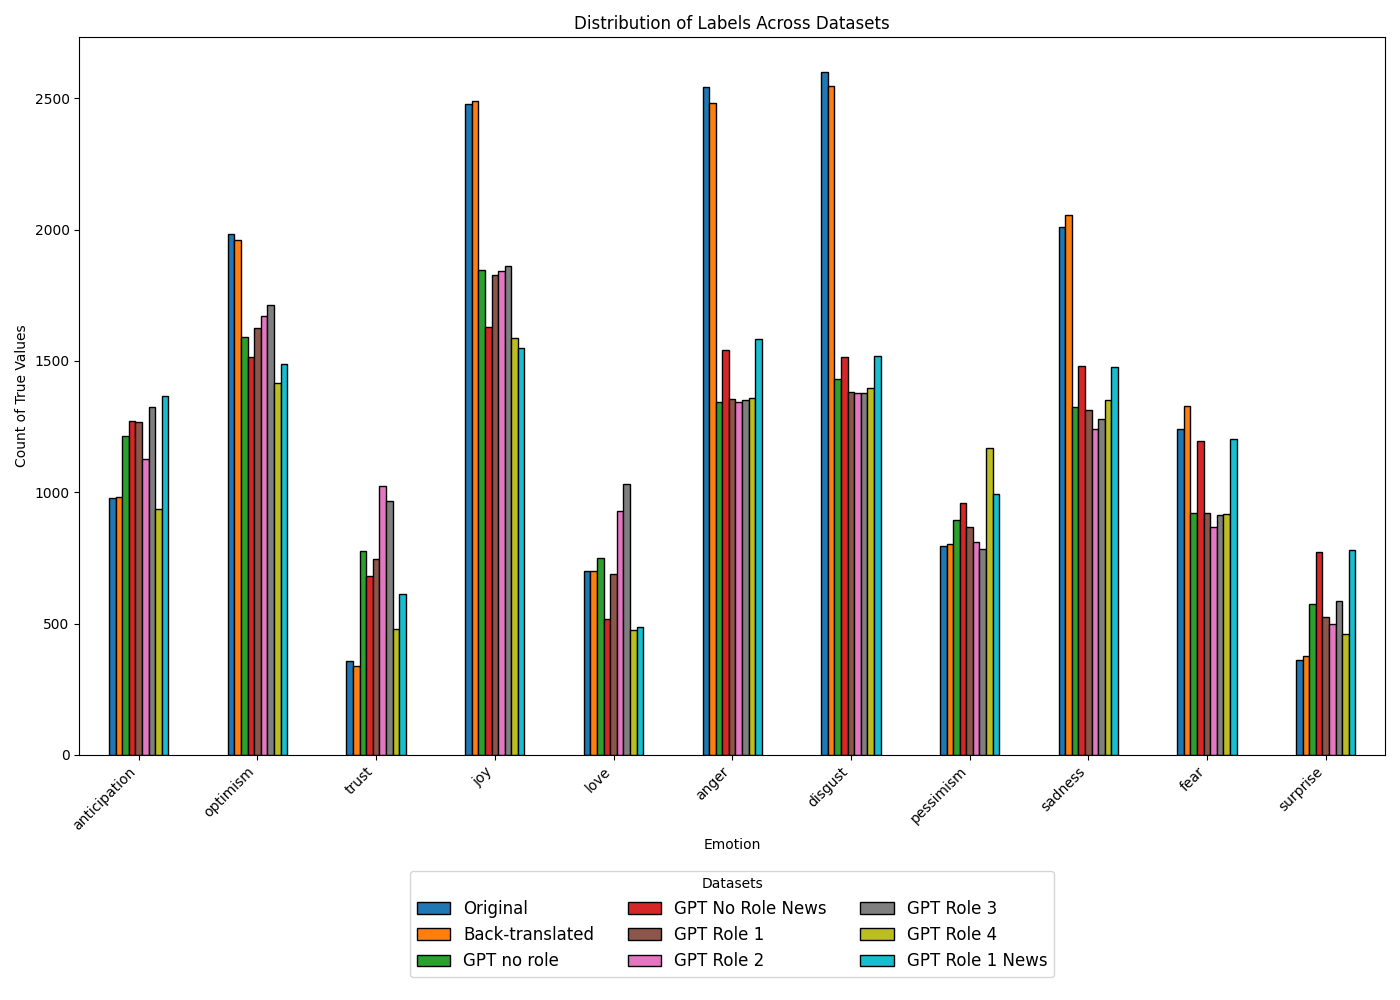
\includegraphics[width=1\linewidth]{label_distribution_comparison.png}
    \caption{Label Distribution in the Gold Standard Data and Augmented Data (Back-Translation and GPT)}
    \label{fig:fig1}
\end{figure}

Furthermore, \autoref{fig:fig2} represents the distribution of data in several additional augmented datasets, which consist of single-label data generated by the GPT model combined with half of the gold standard data. This means that only one label for which the tweets were generated, was tagged as "True", with the other classes tagged as "False". For this data, the distribution is the same as for the the gold standard, since almost all of the labels were augmented by the same number of examples - 100. The lower overall number of instances can be explained by the fact that only half of the gold standard data is augmented with synthetic data. Slight fluctuations in the generated datasets can also be explained by the fact that certain data samples generated by the GPT model featured multiple labels despite explicit instructions to limit the labeling of data to a single "True" emotion. Nevertheless, these instances were rare in the synthetic data.

\begin{figure}
    \centering
    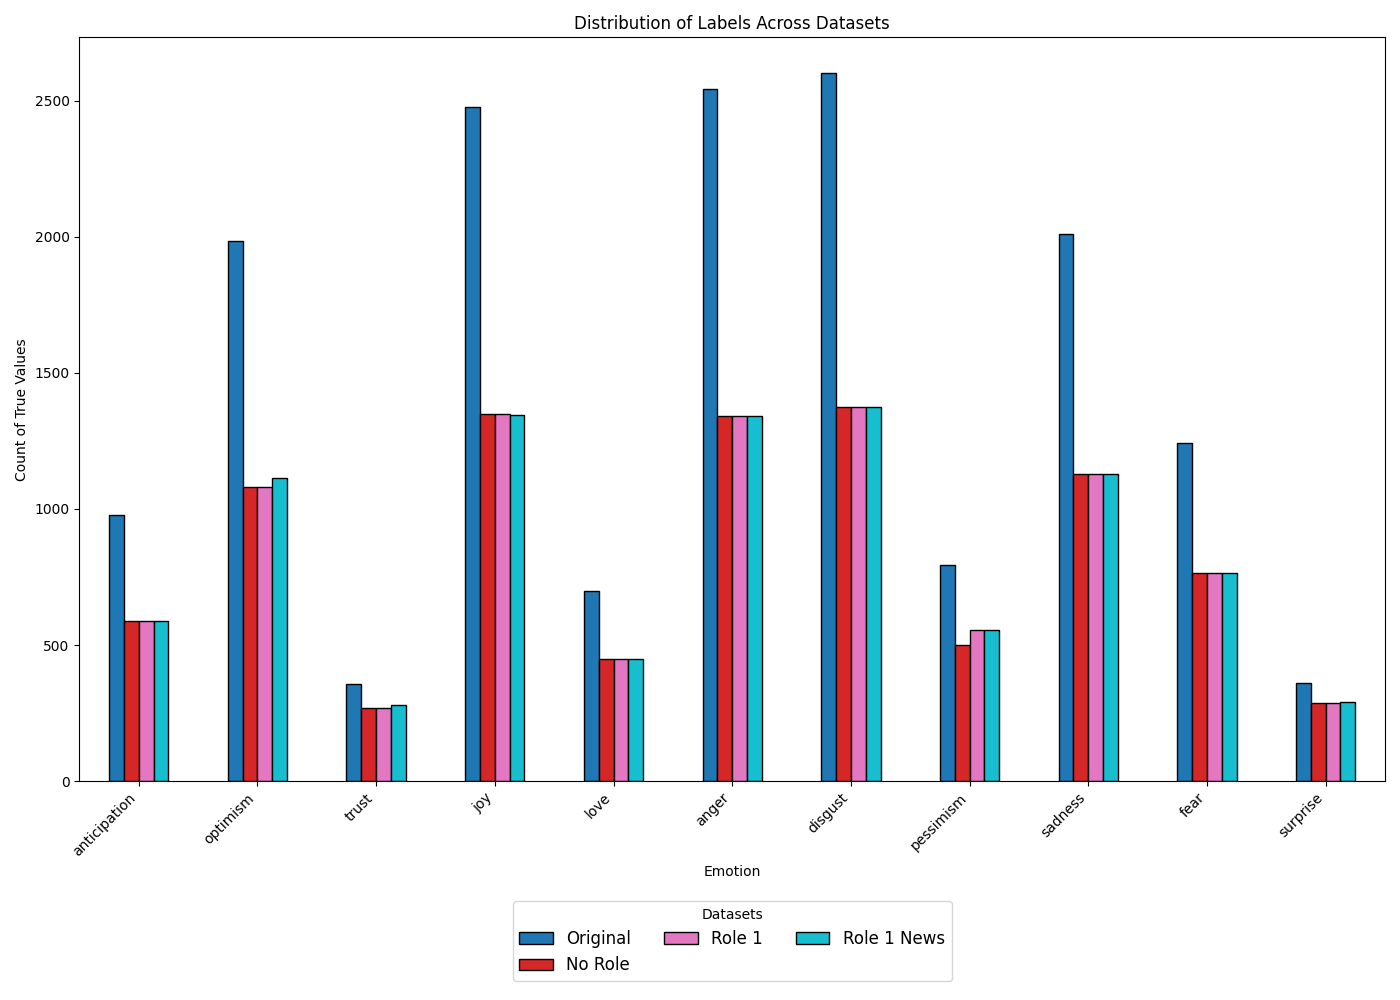
\includegraphics[width=1\linewidth]{single_label_distribution_comparison.png}
    \caption{Label Distribution in the Gold Standard Data and Augmented Single-label Data (GPT)}
    \label{fig:fig2}
\end{figure}

\subsection{Back-Translation Baseline}
Similarly to the research of \citet{van-nooten-daelemans-2023-improving}, we opted for back-translation as the baseline for the experiment. To create the augmented dataset, we selected half of the gold standard data. This approach helps maintain the original label distribution in the augmented dataset while reducing the computational cost of back-translation. Additionally, selecting half of the dataset enables a more accurate evaluation of the DA technique's improvement over the baseline. Subsequently, we translated the tweets from English to French and back to English with the Google Translate's neural machine translation model. The resulting back-translated set of tweets was then merged with the slice of gold standard data and used as the augmented dataset. It was expected that this process would introduce paraphrases and linguistic variations, potentially enriching the training data and improving model performance.

\subsection{Generated Data}
The distributions of the gold standard data and the data generated through Google Translate and GPT model had some differences, which is illustrated in \autoref{fig:fig1}. The synthetic data generation method using the GPT model also introduced certain difficulties, since each instance was generated separately and requested to be multi-label. This means that only the minimum number of instances of a certain label was controlled. This number was set to 100 examples, and was then naturally increased to varying extents as the model generated examples for other labels. This way, we generated 1,100 tweets with corresponding labels for the augmentation of our data. This number was chosen with the expectations to have a sufficient number of examples, which could be represented in the training outcome. The data was generated using three approaches: role-free generation, role-based prompting, and role-based prompting with news headlines (see \autoref{appendix}), as further described in \autoref{prompt} on Prompt Engineering. All the approaches are also summarized in \autoref{tab:approaches}. Afterwards, the synthetic data was combined with half of the gold standard data for the experimentation. Additional analysis was carried with a combination of complete gold standard data and synthetic generated data.

To investigate the influence of different generation methods on data quality, we generated 100 single-label tweets for each emotion category. In other words, only one label was tagged with "True", and the rest were "False". This part was done re-using the three distinct approaches that were applied to generate multi-label data. This additional experimentation allowed us to compare the effectiveness of a variety of methods in augmenting training data. For this analysis, we also used two approaches: combining the data with half of the original dataset, and the complete gold standard dataset.

Finally, to further investigate the impact of synthetic data quantity on model performance, we expanded the dataset by generating additional examples without roles for both multi-label and single-label tweets. 200 tweets were generated for each label, resulting in 2 200 additional tweets that were added to the half of gold standard data to measure the impact. This experiment aimed to assess the influence of increased data volume on model performance in comparison to the back-translation baseline while simultaneously comparing the effectiveness of role-based prompting. This was done combining the synthetic data with half of the gold standard dataset.

\begin{table}
    \centering
    \begin{tabular}{ccccc}
           Label Type&  Role Inclusion&  News Data&  Examples per label &Avg. labels/tweet\\
           multi-label&  no role&  No&  100 &4.22\\
           multi-label&  no role&  Yes&  100 &4.59\\
           multi-label&  role 1&  No&  100 &4.10\\
           multi-label&  role 2&  No&  100 &4.33\\
           multi-label&  role 3&  No&  100 &4.72\\
           multi-label&  role 4&  No&  100 &3.21\\
           multi-label&  role 1&  Yes&  100 &4.63\\
           single-label&  no role&  No&  100 &1\\
  single-label& role 1& No&100 &1\\
  single-label& role 1& Yes&100 &1\\
           multi-label&  no role&  No&  200 &4.23\\
  single-label& no role& No&200 &1\\
    \end{tabular}
    \caption{The approaches to generating data with GPT-4o-mini model. Each dataset, except those with 200 examples per label, was combined with either half of the gold standard data, or complete gold standard dataset, and was subsequently used to train both BERT and RoBERTa models.}
    \label{tab:approaches}
\end{table}

\subsubsection{Prompt Engineering} \label{prompt}
Following the insights of \citet{yoo2021gpt3mix} on effective GPT prompting, we design prompts that include both a description of the labels and an example drawn from the gold standard data with a single label representative of the emotion. This one-shot learning approach aims to provide sufficient context for the model to generate accurate emotion labels for new instances. 

The examples for the model are drawn from the gold standard data based on cosine similarity. By using this metric, we intended to identify examples that are semantically closest to the target label. This was done in order to provide examples that would be most representative of their respective labels. For all labels except '\textit{trust}', the single-label example was taken. Since there were no tweets labeled with only '\textit{trust}', a multi-label example had been selected separately based on the same metric. An additional condition was introduced for the '\textit{anger}' tweet, which meant that the minimal length of the tweet had to be at least 5 tokens. This was done to give the GPT model more context and avoid short tweets, such as '\textit{I am angry}'.

The prompt was comprised of three key elements: label definitions, instructions relevant to the task, and a tweet example taken from the gold standard dataset. First, we introduce the model to the target label, prompting it to generate a corresponding example. To guide the model, we supply a pre-selected relevant example, as shown below:
\begin{example}
\textit{Given the following label: disgust (also includes disinterest, dislike, loathing) \newline
Generate a tweet for the emotion: disgust. Ensure that other appropriate emotions (anger, anticipation, disgust, fear, joy, love, optimism, sadness, surprise, trust) are also present in the tweet that you generate. The disgust label must be tagged as 'True'. The tweet should be stylistically similar to the example below: \newline
I don't like pineapple I only eat them on pizza, they lose the sting when they get cooked.}
\end{example}
Subsequently, we include system prompts for the DA by incorporating roles based on the OCEAN model. Two of the roles included random values for all traits, and two other prompts instantiated all equal values (all HIGH or all LOW). The overview of all roles can be seen in \autoref{tab:roles_values}. For the first two roles, the traits were given one of three values, as in the example below:
\begin{example}
\textit{You are a person who received the following results on the Big Five Personality test: \newline
Openness: HIGH \newline
Conscientiousness: MEDIUM \newline
Extraversion: LOW \newline
Agreeableness: LOW \newline
Neuroticism: MEDIUM}
\end{example}
The prompt to the GPT-4o-mini model was thus adjusted to take into account the system prompt:
\begin{example}
\textit{Given the following label: disgust (also includes disinterest, dislike, loathing) \newline
Generate a tweet in accordance with your personality score for the emotion: disgust. Ensure that other appropriate emotions (anger, anticipation, disgust, fear, joy, love, optimism, sadness, surprise, trust) are also present in the tweet that you generate. The disgust label must be tagged as 'True'. The tweet should be stylistically similar to the example below: \newline
I don't like pineapple I only eat them on pizza, they lose the sting when they get cooked.}
\end{example}
To further explore the impact of external stimuli on the output of the GPT model, we incorporated 20 headlines from BBC articles dated August 6, 2024, into our prompts \autoref{appendix}. The headlines were selected manually at random, with the main focus being on diversity of topics. This approach aimed to induce more varied and creative responses by exposing the model to relevant and potentially provocative topics. To establish a baseline, we initially generated tweets without any role-specific prompts, followed by experiments using one of our pre-defined role-based prompts: 
\begin{example}
\textit{Given the following label: disgust (also includes disinterest, dislike, loathing) \newline
Generate a tweet for the emotion: disgust. The tweet should be on the topic of this news headline: Biden meets national security team as fears of Iran attack on Israel grow. Ensure that other appropriate emotions (anger, anticipation, disgust, fear, joy, love, optimism, sadness, surprise, trust) are also present in the tweet that you generate. The disgust label must be tagged as 'True'. The tweet should be stylistically similar to the example below: \newline
I don't like pineapple I only eat them on pizza, they lose the sting when they get cooked.}
\end{example}
As for the additional single-label data generation, prompts were modified to explicitly require the model to output text expressing a single, specified emotion and to refrain from labeling other emotions as 'True', resulting in the following prompt:
\begin{example}
\textit{Given the following label: disgust (also includes disinterest, dislike, loathing)\newline
Generate a tweet in accordance with your personality score for the emotion: disgust. Ensure that only the label for disgust is True. The tweet should be stylistically similar to the example below:\newline
I don't like pineapple I only eat them on pizza, they lose the sting when they get cooked.}
\end{example}
The prompt was modified in analogous ways to multi-label tweet generation to include a role or feature news headlines as topics.

\subsubsection{Label Description} To guide the GPT-4o-mini model in generating tweets aligned with the labels in the data, we leveraged the label descriptions from \citet{mohammad-kiritchenko-2018-understanding}. These descriptions were originally provided to human annotators tasked with determining the emotional state of tweets' authors. In our analysis, the label descriptions served as a foundation for prompt construction. The model was provided with the corresponding label description for each emotion it was generating tweets for.
\subsubsection{Task Description: Data Augmentation} The GPT model was instructed to generate additional examples of the data based on the label descriptions and, in some instances, the attributed role. Due to the explicit instructions to generate multi-label data, the distribution of the gold standard data was altered. However, the specific number of generated data entries was chosen as a balance between computational efficiency, cost considerations and the potential for significantly enhancing classification performance. Leveraging the provided label descriptions, assigned roles and examples, the model was prompted to create diverse and contextually relevant tweet instances. This augmentation strategy aimed to enrich the dataset with synthetic examples that capture the underlying patterns and variations present in the original data. The data was then combined with either half or complete gold standard data for the classification part of the experiment.
\subsubsection{Role Attribution} This work builds upon the concept explored by \citet{hilliard2024elicitingpersonalitytraitslarge} of a technique for incorporating OCEAN model's personality traits into GPT prompting for DA. We first established a baseline of generating tweets with no role attributed. Subsequently, each category within the OCEAN model was assigned a ranking (HIGH, MEDIUM, or LOW) to influence the GPT model's outputs. The role was given as a system prompt, and was referred to in the user prompt. A total of four distinct roles was employed, with an additional condition combining the first role with BBC news headlines. 
\subsubsection{Example Selection} In order to enhance control over the generated data and provide the classification models with clear instances of target emotions, a single representative example was selected for each label based on cosine similarity and additional previously described criteria. Specifically, for each label, we filtered out multi-label examples and selected only those tweets that expressed a single emotional category. Cosine similarity was calculated between the vector representations of tweets, and for each emotion, the tweet with the highest average similarity to all other tweets within the same emotional category was selected. This process ensured that the selected examples not only aligned with the correct emotional category but also exhibited strong stylistic consistency within the label. By selecting tweets with high intra-label similarity, we aimed to guide the GPT-4o-mini model towards generating text that accurately reflected both the target emotion and the stylistic characteristics of the original dataset, thereby improving the quality and relevance of the generated data. Examples of the synthetic data for each label can be seen in \autoref{all_examples}.

\subsection{Classification Models}
\subsubsection{Baseline}
We employed a Support Vector Machine as the baseline classifier, evaluating its performance under the OneVsRestClassifier problem transformation approach. The tweets were transformed using a TfidfVectorizer with the limit of maximum features equal to 5,000. For this model, the train set was concatenated with the validation set to enhance training robustness.
\subsubsection{LMs}
To facilitate the comparison, we additionally included LMs as baseline models for the experimental results: \textbf{BERT} and \textbf{RoBERTa}. These models were chosen as baselines due to their widespread adoption and proven effectiveness in various NLP tasks, allowing us to benchmark our results against well-established standards in the field.

Each model was trained with four different inputs: half of the gold standard data, the entirety of the gold standard data, half of the gold standard data combined with the augmented data, and full gold standard dataset with the augmented data (\autoref{tab:baseline_results}). To create the balanced subset of the gold standard data, the training section of the dataset was partitioned while preserving the original class distribution as closely as possible \cite{10.1007/978-3-642-23808-6_10}, accounting for the multi-label nature of the data. To mitigate the potential impact of random initialization on model performance, three different random seeds were employed for training the classification models (42, 1410, 1995). This was done for the training of BERT and RoBERTa models.

The hyperparameters for each model were selected based on a combination of empirical experimentation and established best practices in the field. As such, all BERT models were trained for 5 epochs, and RoBERTa models were trained for 10. We selected the best performing model based on its validation loss. A learning rate of 1e-5 and a dropout rate of 0.2 were employed during training. Batch sizes were set at 32 for both models, but gradient accumulation steps of 4 were used for RoBERTa due to computational limitations. The optimizer used for both models was AdamW, following the original implementation of BERT \cite{DBLP:journals/corr/abs-1810-04805}.

\subsection{Generative Model Parameters}
For the GPT-4o-mini completion model, the temperature was set to 0.7, and the 'top p', 'frequency penalty' and 'presence penalty' were all set to 1. Finally, the maximum generated tokens was set to 200.

For the establishment of a baseline, no system prompts were employed for data augmentation. Subsequently, system prompts were introduced to imbue the models with specific roles. Additionally, to ensure consistency and facilitate downstream processing, generated examples were formatted as JSON objects using function calling. The description of the function also included the mention of the average length of the tweets - 16 tokens.
\subsection{Model Evaluation}
The performance of each model is reported based on exact match ratio (EMR), which measures the proportion of instances where the predicted labels align with the ground truth labels. In addition, F1-macro and F1-micro scores were computed to assess and compare the models' performances. As previously mentioned, to ensure a robust evaluation, experiments were conducted using three different random seeds, and the reported results represent the average performance along with the standard deviation across the seeds. The standard deviation helps to determine the stability of reported results. The models were assessed using the aforementioned metrics to evaluate their ability to accurately classify emotions. Due to computational limitations, the BERT and RoBERTa models trained on combinations of gold standard data and GPT-generated data were evaluated using a single seed (42). 

\section{Results and Discussion}
This section presents a comprehensive analysis of the results of our experiments, including the performance of models trained on augmented data. First, the effects of DA on multi-label classification will be discussed. Following this analysis, we discuss the insights from additional experiments conducted. To gain deeper understanding of the quality of the synthetic data and the underlying generative process, we conducted a typicality analysis comparing human-authored and synthetic text. The classification reports can be accessed on GitHub repository through the Appendix \autoref{repo}
\subsection{Effect of Data Augmentation}
\autoref{tab:baseline_results} illustrates the performance of each model across different data conditions. The abbreviation GSD in the table denotes the gold standard data. In line with the expectations, SVC underperformed compared to the other models, despite the addition of the validation set to the training data. Additionally, while DA yielded some modest performance gains over the sample of the gold standard data, the improvements were not consistent and fell short of the gold standard benchmark. It can also be seen that RoBERTa outperformed BERT across all data conditions. This difference could be explained by the model's pre-training, allowing it to capture more nuanced patterns in the data, and resulting in better generalization across diverse data conditions compared to BERT.

It is worth mentioning that none of the baseline models reached the previous state-of-the-art results of \citet{baziotis2018ntuaslp}: accuracy of 58.8\%, F1-micro of 70.1\% and F1-macro of 52.8\%, or the results of \citet{10.1016/j.eswa.2022.118534}: accuracy of 62.4\%, F1-micro 74.2\% and F1-macro 60.3\%. Given that the comparison is made against established SOTA models, it is expected that the baseline models, especially when trained on slices of gold standard data, would not surpass these benchmarks. However, \autoref{full_gsd_results} shows the results for the models trained on complete original data that had been augmented. In this setting, the results were much closer to the benchmark.

The comparative analysis of BERT models under varying data conditions reveals distinct performance patterns. While all models exhibited strong accuracy in predicting the absence of "\textit{trust}" and "\textit{surprise}" labels, their proficiency in classifying other emotions varied significantly. This might indicate the models' hesitance to predict underrepresented labels, thus highlighting the need for more data. In line with expectations, using half of the gold standard data led to a decline in overall performance compared to the full dataset, which is particularly evident in the increased false positive rates for emotions like "\textit{optimism}" and "\textit{anger}". Overall, the performance of these models reaffirms the findings of \citet{10.1016/j.eswa.2022.118534}, which were based on models trained with the full training data, regarding the difficulties the model encounters with particular classes. The integration of synthetic back-translated data did not produce consistent improvements in performance, suggesting that the quality and relevance of synthetic data might be crucial factors in achieving performance gains.

The results for the RoBERTa models closely resemble the patters that were observed for the BERT models. However, the integration of synthetic back-translated data yielded mixed results, with slight improvements in some emotion categories, such as "\textit{joy}" and "\textit{anticipation}", but declines in others relative to the original dataset, such as "\textit{fear}" and "\textit{sadness}". It could also be seen that the model completely failed to identify any instances of the "\textit{trust}" or "\textit{surprise}" labels, resulting in all positive instances being classified as negative. This indicates that the model has severe issues with recognizing these labels, which were the classes with the least occurrences in the entire dataset. The absence of false positives suggests that the model doesn't mistakenly classify any negative instances as "\textit{trust}" or "\textit{surprise}", but this remains suboptimal given the complete lack of true positives. 
\begin{table}
    \centering
    \begin{tabular}{lcccc}
          Classifier&GSD proportion&  Accuracy (SD)&  F1-micro (SD)&  F1-macro (SD)\\
         SVC&100\%&  18.04&  55.20&  37.94 \\
         BERT&50\%&  25.73 (0.38)&  66.06 (0.63)&  42.33 (1.39)\\
         BERT&100\%&  28.54 (0.05)&  68.82 (0.09)&  48.57 (0.69)\\
 BERT + back-translation&50\%& 26.80 (0.76)& 67.92 (0.68)& 48.81 (0.66)\\
 RoBERTa&50\%& 26.78 (0.28)& 67.18 (0.72)& 44.32 (1.00)\\
 RoBERTa&100\%& 28.95 (0.51)& 70.26 (0.47)& 50.92 (0.83)\\
 RoBERTa + back-translation&50\%& 28.54 (0.20)& 69.67 (0.21)& 50.47 (0.85)\\
 \multicolumn{5}{c}{Multi-label GPT-generated data (no role)}\\
 BERT&50\%& 26.08& 67.06& 49.12 \\
 RoBERTa&50\%& 22.31& 66.42& 51.49 \\
 BERT& 100\%& 27.19& 68.75& 52.46\\
 RoBERTa& 100\%& 27.31& 70.15& 53.76\\
 \multicolumn{5}{c}{Doubled multi-label GPT-generated data (no role)}\\
 BERT& 50\%& 25.71& 67.47&49.70\\
 RoBERTa& 50\%& 24.42& 67.58&52.58\\
 \multicolumn{5}{c}{Single-label GPT-generated data (no role)}\\
 BERT& 50\%& 26.08& 66.65&44.53\\
 RoBERTa& 50\%& 26.02& 66.87&45.97\\
 BERT& 100\%& 27.31& 67.91&50.85\\
 RoBERTa& 100\%& 27.95& 69.43&52.39\\
 \multicolumn{5}{c}{Doubled single-label for GPT-generated data (no role)}\\
 BERT& 50\%& 25.35& 66.13&45.81\\
 RoBERTa& 50\%& 25.50& 67.15&49.97\\
    \end{tabular}
    \caption{The Evaluation of Baseline Models}
    \label{tab:baseline_results}
\end{table}

On the other hand, while the BERT model trained on the GPT-generated data with no explicit role attribution and half of the gold standard data achieved similar performance to the BERT trained on back-translated data, it nevertheless exhibited more struggles in certain categories, namely "\textit{trust}", "\textit{anticipation}" and "\textit{surprise}". Nevertheless, taking into consideration the improvements over the BERT using half of the GSD, the GPT data suggests some compatibility with the gold standard. However, despite an increase in instances of underrepresented labels within the augmented dataset, the model did not exhibit a corresponding improvement in performance for these classes, suggesting potential limitations in leveraging synthetic data for addressing class imbalance. These results also highlight the fact that the multi-label synthetic data generated by the GPT model may not be superior to the back-translated data. It is nevertheless worth noting that the comparable results were achieved with GPT-generated data with substantially fewer examples than those achieved with back-translated data. The results for the doubled multi-label GPT data suggest a better performance.

The performance characteristics of RoBERTa models trained with augmented data revealed patterns that were contrasting with those obtained for BERT. While RoBERTa trained on the GPT data without role attribution achieved markedly lower accuracy and F1-micro scores compared to all other LMs, it nevertheless achieved a slightly higher F1-macro score. This result could potentially indicate that the model is better at predicting minority classes or balancing predictions across classes, despite its lower overall accuracy. This could be seen in the predictions made for the problematic "\textit{trust}" and "\textit{surprise}" labels. While the model still demonstrated poor performance with these classes, it was able to predict a few true positives. This improvement does not overshadow the fact that the model struggles to correctly classify many instances of "\textit{trust}" or "\textit{surprise}" and has a high number of false positives. Overall, this indicates that the GPT-generated data is somewhat useful in addressing the data imbalance issue. 

Proceeding with the analysis, additional results for the single-label DA can be seen in \autoref{tab:baseline_results}, which show the evaluation of BERT and RoBERTa models when trained on a combination of GPT-generated single-label data with no role attribution and gold standard data. 

In comparison to the multi-label generated data, the results for single-label BERT are almost identical, with slightly better F1-micro and moderately higher F1-macro achieved on multi-label data. Conversely, the performance of RoBERTa is more nuanced. The RoBERTa model performs better on "\textit{love}", "\textit{joy}" and "\textit{optimism}" categories when trained on single-label data, while multi-label examples allowed the model to perform better on "\textit{disgust}", "\textit{sadness}" and "\textit{pessimism}". While the performance of both models is suboptimal, a possible explanation for such results could be linked to emotions like \textit{love}, \textit{joy}, and \textit{optimism} often being expressed in more distinct and positive contexts, which could be easier for the model to recognize when trained on single-label data. On the other hand, emotions like \textit{disgust}, \textit{sadness}, and \textit{pessimism} might overlap with other emotions or be expressed in more nuanced ways, benefiting from the multi-label training that allows the model to see these emotions in conjunction with others.

Following the analysis, additional experimentation was done to evaluate the effect of GPT-generated data on multi-label classification tasks. For that, we doubled the size of the generated data and used it along with the sample of the gold standard dataset for evaluation. The results of this experiment can be seen in \autoref{tab:baseline_results}.

While there were some improvements, the results suggest that doubling the amount of generated GPT data did not lead to clearly improved results in the task. It is possible that the model's performance reaches a plateau, likely due to data homogeneity. This suggests that the generated data lacks sufficient variation to enable the model to acquire new knowledge during training. The only notable results were achieved by the RoBERTa model trained on multi-label synthetic data, which reached improvements in all three metrics, and even surpassed the F1-macro score of the RoBERTa model trained only on gold standard data. However, the reason for the lack of improvements in other cases could be attributed to data quality and model generalization. While increasing data volumes can enhance model performance by providing more diverse examples, it is crucial that the additional data is both relevant and representative of the real world. In this case, the supplementary generated data may have introduced more noise or lacked the contextual accuracy necessary for effective classification, therefore hindering the model's ability to learn meaningful patterns. If the doubled dataset contained redundant or less informative examples, the model's learning process could be diluted, leading to diminished returns in classification results. Hence, the inefficacy of merely increasing the dataset with the help of a GPT model highlights a limit to the usefulness of GPT-produced synthetic data. It also shows the need for a more balanced approach that prioritizes both the relevance and diversity of data to truly enhance model performance.

Based on these baseline results, our findings suggest that the comparable performance of models trained on gold standard data and back-translated data indicate the value of DA as a viable complement to the gold standard, albeit with marginally reduced effectiveness. These findings underscore the challenges associated with generating high-quality synthetic data.

\subsection{OCEAN Role Impact}
To further explore the potential of GPTs for DA and role-based prompting, we analyze the data for which GPT-4o-mini model was assigned specific personality scores based on the OCEAN model. The values used for each role can be seen in \autoref{tab:roles_values}. By manipulating these underlying personality dimensions, we aimed to induce variations in the generated text and assess the impact on downstream classification tasks.

\begin{table}
    \centering
    \begin{tabular}{cccccc}
         Role&  Oppenness&  Conscientiousness&  Extraversion&  Agreeableness& Neuroticism\\
         role 1&  MEDIUM&  LOW&  HIGH&  LOW& HIGH\\
         role 2&  LOW&  MEDIUM&  MEDIUM&  HIGH& LOW\\
         role 3&  HIGH&  HIGH&  HIGH&  HIGH& HIGH\\
         role 4&  LOW&  LOW&  LOW&  LOW& LOW\\
    \end{tabular}
    \caption{Values for the roles employed in generating data with the GPT model}
    \label{tab:roles_values}
\end{table}

The examples of tweets can be found in \autoref{all_examples}. Some obvious differences can be observed when comparing the data featuring news articles to that without it. However, the inclusion of roles does not seem to produce particularly diverse examples.

A comparative analysis of classification performance for BERT and RoBERTa models utilizing GPT-augmented data is presented in \autoref{tab:role-based_BERT} and \autoref{tab:role-based_RoBERTa} respectively. 

Based on our hypothesis that specific OCEAN personality profiles would be associated with particular text generation patterns, our results provide insights into whether this idea can be supported. The comparison of the evaluation metrics across all data modalities reveals little difference in achieved results, suggesting minimal effect of role attribution on augmented data. It must also be mentioned that part of the fluctuation could be attributed to the fluctuations in data distribution across the combined datasets.
\begin{table}
    \centering
    \begin{tabular}{cccc}
         &  accuracy&  F1-micro& F1-macro\\
         no role&  26.08&  67.06& 49.12\\
 no role + news& 25.71& 67.39&48.50\\
         role 1&  25.31&  65.67& 46.32\\
         role 2&  26.27&  66.44& 46.64\\
         role 3&  25.68&  66.53& 47.64\\
         role 4&  26.51&  67.47& 48.18\\
         role 1 + news&  25.77&  67.13& 49.61\\
    \end{tabular}
    \caption{The Evaluation of the Role-based Data Generated by GPT-4o-mini on BERT}
    \label{tab:role-based_BERT}
\end{table}

The results for the BERT model suggest that the performance of models on role-based datasets, including those featuring news articles, is highly similar to the dataset with no role attribution. However, it could be seen that the tendency of higher F1-macro score remains, indicating that the data likely aided the model to predict underrepresented labels. While these results are also similar to those achieved by the model trained on back-translated data, it is worth mentioning that an improvement over the baseline model trained on half of the data was achieved. For this model, the best accuracy and F1-micro scores were achieved for role 4, role-based data, for which all of the personality traits were set to a LOW score. While the F1-macro score is also relatively high on this dataset, the highest evaluation was achieved on the dataset based on role 1, a prompt with mixed trait evaluations, combined with news article topics.

\begin{table}
    \centering
    \begin{tabular}{cccc}
         &  accuracy&  F1-micro& F1-macro\\
         no role&  22.31&  66.42& 51.49\\
 no role + news& 25.81& 67.90&52.02\\
         role 1&  24.42&  66.93& 51.05\\
         role 2&  24.39&  67.25& 51.56\\
         role 3&  22.74&  65.88& 50.31\\
         role 4&  26.08&  68.19& 51.73\\
         role 1 + news&  26.11&  67.91& 51.46\\
    \end{tabular}
    \caption{The Evaluation of the Role-based Data Generated by GPT-4o-mini on RoBERTa}
    \label{tab:role-based_RoBERTa}
\end{table}

As for the results shown in \autoref{tab:role-based_RoBERTa}, while RoBERTa exhibited performance trends similar to those of BERT, certain differences emerged upon closer examination. One clear difference is the improvement of the majority of evaluation metrics demonstrated over the no-role baseline, with subtle variations observed in specific instances. Similarly to BERT, data generated with role 4 yielded the highest F1-micro score, and relatively high scores for other metrics. It can also be seen that data featuring role 1 and news articles achieved elevated scores, yielding the highest accuracy score for this subset of datasets for RoBERTa. Finally, the highest F1-macro score was achieved on the data that was generated without a role, but featured article headlines. 

This analysis of BERT and RoBERTa reveals subtle yet notable trends in how role-based data influences model performance. Both models demonstrate that integrating GPT data, with or without specific personality traits, can marginally enhance predictive accuracy, especially in underrepresented labels compared to baselines with and without synthetic data, as indicated by the consistently higher F1-macro scores. Interestingly, the role-based prompt associated with uniformly low personality scores (Role 4) consistently yielded the highest F1-micro scores for both BERT and RoBERTa models. This suggests that the models might benefit from more uniform data provided by this role configuration to a certain degree, leading to more consistent predictions. Additionally, the inclusion of news articles and mixed role evaluations in role 1 data appears to contribute positively to the models’ performance, with RoBERTa achieving its highest accuracy on this subset. The RoBERTa model’s highest F1-macro score, however, was achieved with a dataset devoid of role attribution but containing article headlines, implying that the absence of role-based features, combined with specific content types, may allow the model to generalize better across varied categories. Although these improvements are marginal, they suggest that role-based data, similarly to GPT-generated data with no role attribution, particularly when combined with relevant contextual content like news articles, can enhance model performance. This is especially evident for underrepresented classes. 

However, the improvements of accuracy are not comparable to those achieved on the gold standard data, or even the back-translation baseline. As for the F1-micro score, while lacking stability, the models seem to reach and even exceed the results of the baselines when trained on GPT-generated data. The main improvement demonstrated by RoBERTa models is evident in F1-macro score, which is also true for the BERT model. This seems to be a general trend inherent to the synthetic data generated through the GPT model, which thus cannot be attributed to role-based prompting.

To further delve into the analysis, \autoref{tab:single_role-based} illustrates the results of BERT and RoBERTa models on single-label generated data. These datasets also include role-based prompting and topics of news articles.

\begin{table}
    \centering
    \begin{tabular}{cccc}
         &  accuracy&  F1-micro& F1-macro\\
 BERT + no role& 26.08& 66.65&44.53\\
         BERT + role 1&  26.76&  66.28& 45.68\\
         BERT + role 1 + news&  26.48&  65.60& 44.55\\
 RoBERTa + no role& 26.02& 66.87&45.97\\
         RoBERTa + role 1&  26.39&  67.40& 48.25\\
         RoBERTa + role 1 + news&  26.88&  67.21& 46.78\\
    \end{tabular}
    \caption{Evaluation of BERT and RoBERTa on role-based single-label data generated by GPT-4o-mini, compared to the no role baseline}
    \label{tab:single_role-based}
\end{table}

The results for the data generated with single labels reveals additional insights into the influence of roles on synthetic tweets. To begin with, the increase in the metrics is more predictable, which most likely stems out of the distribution of the data. This means that unlike the case for the multi-label augmentation, the underrepresented classes are less affected by augmented data with single "True" labels. One possible reason is insufficient targeting of minority classes by single-label augmentation, as it lacks the complexity of multi-label augmentation, where multiple emotions can be addressed simultaneously, potentially offering more opportunities for the rare classes to be represented. Additionally, it is possible that due to vagueness of certain emotions, the model tends to include them more often into the generated data. One predominant trend is the steady increase in most metrics when introducing role-based data. While most improvements are modest, especially for the BERT model, they are nevertheless consistent in comparison to the single-label data generated without role attribution. In addition, it could be noted that models performed best on role 1 data without news articles, which is applicable for both BERT and RoBERTa.

When comparing the single-label to multi-label generated data (\autoref{tab:role-based_BERT}, \autoref{tab:role-based_RoBERTa}, \autoref{tab:single_role-based}), the single-label data, for the most part, achieves lower performance compared to synthetic multi-label data. However, the accuracy of BERT is highest when trained on single-label role 1 dataset than any other GPT-generated data. This is also true for RoBERTa model, both with and without news article headlines. Contrary to multi-label data evaluation, this part of the experiment highlights with slightly more clarity the potential benefits of incorporating mixed role evaluations and context-rich content like news articles. This also suggests that, despite the general advantages of multi-label training, carefully curated single-label data can offer significant performance gains under specific conditions. 

Contrary to initial expectations, this analysis suggests that the integration of role-imbued GPT-generated data into the training process of BERT and RoBERTa does not yield significant performance improvements. The results for multi-label augmentation consistently demonstrate that models trained on datasets with more traditional approaches to DA outperformed those incorporating role-specific prompts. One possible explanation is the cause of guardrails imposed on the model during RLHF, preventing the change in the manner in which the model generates data. These findings challenge the hypothesis that imbuing language models with specific personality traits would substantially enhance DA strategies and, consequently, downstream task performance. Nonetheless, the results achieved on the data with single-label augmentation suggests that there might be some benefit to role-based prompting, which is why the hypothesis cannot be fully dismissed.

\subsection{Data Typicality}
To better understand the effects of GPT-4o-mini and the roles it was attributed, we measured the typicality of data \cite{ZHANG1992470}. In essence, data typicality is a measure of how well a data point or dataset reflects the underlying patterns and trends within the data. This metric is particularly valuable for evaluating synthetic data, as it allows us to assess how closely the generated examples align with the distribution and characteristics of the original training data. Furthermore, we evaluated how different the GPT-generated data is when generating synthetic data directly compared to when the model is explicitly attributed a particular personality. To quantify this, we compute the data typicality using cosine similarity \cite{van-nooten-daelemans-2023-improving}, as it effectively captures semantic and directional similarities between text data points. Specifically, we measure the average cosine similarity between each generated instance and the gold standard instances from the same label, and then compare it to the average cosine similarity between the generated instance and instances from different labels.
\begin{equation}
\text{Typicality}(\mathbf{g}) = \frac{ \frac{1}{|N(a)_l|} \sum_{\mathbf{x} \in N(a)_l} \text{sim}(\mathbf{g}, \mathbf{x}) }{ \frac{1}{|N(a)_k|} \sum_{\mathbf{x} \in N(a)_k} \text{sim}(\mathbf{g}, \mathbf{x}) }
\end{equation}
The results of this analysis are summarized in \autoref{tab:typicality_multi}. As an additional metric, we calculated Type-Token Ratio (TTR), which represents the measure of lexical diversity in the original and generated texts. This is done by dividing the number of unique words by the total number of words.

\begin{table}
    \centering
    \begin{tabular}{cccc}
         & Overall Typicality  &Length&TTR\\
 GSD&1.23  &20&.12\\
         no role& 1.03  &19&.05\\
         no role + news& 1.02  &24&.06\\
         role 1& 1.03  &18&.06\\
         role 2& 1.03  &19&.05\\
         role 3& 1.03  &19&.05\\
         role 4& 1.02  &18&.06\\
         role 1 + news& 1.02  &22&.07\\
    \end{tabular}
    \caption{Data typicality for multi-label data. The typicality for GSD represents the overall typicality of labels within the dataset, while the values for other datasets are compared to the GSD. The length represents the number of tokens per tweet using NLTK tokenizer}
    \label{tab:typicality_multi}
\end{table}

Additionally, we calculated the typicality for the data generated with a single label (\autoref{tab:typicality_single}). It can be clearly seen that the results for the data generated with a single label are identical to those for multi-label data. On average, the instances from all of the synthetic datasets seem to be slightly more prototypical than the gold standard data, as can be derived from both \autoref{tab:typicality_multi} and \autoref{tab:typicality_single}. These results also closely resemble those achieved by \citet{van-nooten-daelemans-2023-improving}. 

\begin{table}
    \centering
    \begin{tabular}{cccc}
         & Overall Typicality  &Length&TTR\\
         no role& 1.03  &17&.06\\
         role 1& 1.03  &17&.06\\
         role 1+ news& 1.02  &19&.08\\
    \end{tabular}
    \caption{Data typicality for single-label data}
    \label{tab:typicality_single}
\end{table}

Notably, the incorporation of role-specific prompts and media-derived events did not significantly alter this trend. The GPT model appears to excel at generating highly prototypical tweets across all emotions. Thus, as \citet{van-nooten-daelemans-2023-improving} note, this suggests that the generated data is primarily a reflection of the patterns prevalent in the GPT's training data. This over-reliance on prototypical examples may limit the model's ability to capture diversity and nuances, particularly concerning the variability and fine distinction of emotional expressions. Our findings indicate that the challenges inherent to ChatGPT and GPT-3.5 have not been fully resolved in the GPT-4o-mini architecture. Consequently, while the model can produce syntactically correct and semantically plausible tweets, it may struggle to capture the nuanced and context-dependent nature of human emotion expression. 

When comparing the synthetic data to the gold standard, one can note that the typicality for the GSD is the highest. This suggests that, on average, the similarity between examples with a given emotion label and other examples with the same label is higher than the similarity between examples with that label and examples without that label. This tendency is not present in the generated examples, where given labels are not more similar to each other than to examples without the labels. Moreover, there is a clear contrast between the value of TTR for the gold standard and the generated data. The lower TTR suggests that the GPT model might be producing more generic or repetitive text and relying on a smaller set of words to convey meaning, potentially missing the lexical richness found in the gold standard tweets. The inclusion of news articles elevates the value by a small margin, making the data slightly more linguistically diverse. 

As an additional piece of analysis complementing the previous findings, we focused on assessing the typicality of the generated datasets. The results can be seen in \autoref{typtable}. The core of this approach is the measurement of how similar the generated data is in the different synthetic datasets. The results, presented as average typicality scores comparing role-based and non role-based datasets, provide insights into the consistency and representativeness of the generated data across different contexts, thus offering a deeper understanding of the generated datasets' alignment with emotional attributes. A score above 1 indicates that the generated tweets are similar to the other synthetic dataset. Conversely, a score below 1 suggests that the generated tweets may be less indicative of the target emotion, or resemble other datasets less.

These results reaffirm that the generated synthetic datasets exhibit high levels of prototypicality, as evidenced by their close resemblance to datasets with varying roles and those without role attribution. It is worth noting that the dataset based on role 4 demonstrates the most significant difference in scores when compared to other role-based datasets (\autoref{typtable}), possibly also reflecting the high performance in the classification task. This can also be seen from the slightly higher TTR, possibly serving as the cause of those improvements \autoref{tab:typicality_multi}. Despite this, the data for role 4 still exhibits a notable lack of diversity, which could similarly limit the breadth of its applicability. Interestingly, while the scores for datasets incorporating news articles also show a degree of prototypicality, the presence of role attribution does not yield clear differences. These datasets, however, consistently report lower overall scores. This trend may be attributed to the inclusion of more topical and contextually relevant information, which potentially introduces a degree of creativity into the synthetic tweets. Consequently, due to the fact that the generated data displays strong prototypicality, the observed lack of diversity and the relatively lower scores for news-based datasets suggest that enhancing the variety and depth of the generated content could improve overall performance and applicability in classification tasks.

\section{Conclusions}
In this paper, we employed the GPT-4o-mini model to expand our dataset of tweets for the purpose of multi-label emotion classification. By generating multi-label and single-label synthetic data with this model, we introduced an additional layer of complexity to the data augmentation process. More precisely, we incorporated personality trait scores based on the OCEAN model into the prompts, adding a dimension of psychological diversity to the generated content. Additionally, we included news article headlines as thematic elements to further enrich the dataset with varied topics. The augmented dataset was then combined with a sample of gold standard data and utilized to assess the quality and efficacy of this augmentation method. We conducted a comparative analysis of multiple language models to evaluate their performance on a downstream multi-label classification task, determining how well the synthetic data contributed to improving the models' classification capabilities.

Through the results of our experiments, we show that the role-based method for data augmentation may yield certain limited advantages in performance on a multi-label classification task, even when the amount of generated data is limited. Additionally, the multi-label data augmented through a GPT model has consistently yielded improvements for underrepresented classes, highlighting its value for imbalanced datasets. At the same time, the single-label data achieved higher enhancements for classifiers' accuracy score, providing also better control over the distribution of the data. It is nevertheless important to state that the data augmented through GPT-4o-mini did not improve the results achieved on the complete gold standard data, highlighting that the data generated by this model is not yet comparable to human-annotated data. However, the results on complete gold standard data with GPT-augmented data show some improvements, indicating its potential value. Overall, these findings suggest that while synthetic data augmentation can be beneficial, especially in addressing class imbalance, the enhancements may not fully match the quality provided by human-generated data. Future work could explore alternative techniques to improve the ability of synthetic data to closely mimic the complexities of real-world data. Additionally, integrating more sophisticated methods for generating synthetic examples and combining them with other data augmentation strategies may potentially offer greater performance gains and more robust solutions for multi-label classification tasks. 

As for the diversification of synthetic data through the assignment of personality types to an LLM, the experimentation on the GPT-4o-mini seems to provide mostly negative results. The influence of different roles seems to be marginal when evaluated on a downstream classification task. While certain roles showed some improvements over the no-role baseline, these improvements could hardly be confidently attributed to prompted personality traits. Nevertheless, the results for single-label augmentation provided some modest support for the opposite, revealing that an inclusion of a role led to better performance in predictions and slightly more linguistic diversity, regardless of whether news headlines were introduced as well or not. This suggests that while personality types might not significantly enhance overall data diversity or model performance in the context of multi-label classification, they could still offer value in specific scenarios or tasks. However, one of the key challenges in multi-label data augmentation remains the unpredictability of label distribution in synthetic data. Generating balanced data where all label combinations are equally represented would likely require a substantial amount of synthetic data, which is often impractical or infeasible. Future research could explore strategies to address this issue, such as leveraging targeted augmentation techniques that prioritize underrepresented label combinations. Additionally, alternative ways to integrate personality attributes more deeply could be explored, or different methodologies for personality-based prompting and data augmentation could be analyzed, potentially uncovering more benefits or identifying the conditions under which personality types might impact model performance more effectively.

Based on the results presented in this paper, the ability of models to effectively handle a multi-label classification problem characterized by class imbalance is rather limited. Classical machine learning models, such as SVC, seem to be largely unfit for this type of classification. Significantly better results can be achieved by language models such as BERT, the results of which were nonetheless suboptimal. While the best results have been achieved by the RoBERTa model, it nevertheless struggled with underrepresented classes. Even in the cases where data for those classes was augmented, the model was unable to identify more true positives than false ones. This may suggest that the issue mentioned by \citet{10.1016/j.eswa.2022.118534} of limited context may persist despite the addition of synthetic data. Addressing this challenge may require further investigation into alternative methods for data augmentation and model refinement. Future research could explore more sophisticated techniques to improve model performance on imbalanced multi-label classification tasks, possibly integrating advanced strategies for context enrichment or leveraging alternative approaches to handle class imbalance more effectively. 

Certain limitations encountered in this research are important to acknowledge, as these constraints influenced the methodology and execution of the experiments in somewhat significant ways. First of all, due to computational limitations, the scope of experimentation with resource-intensive models such as BERT and RoBERTa was constrained. These limitations restricted the overall number and size of augmented datasets, thereby limiting the exploration of different roles and the variety in their implementation. Additionally, managing the distribution of multi-label data presented challenges, which meant that only the minimum margin of control could be effectively handled. Future work could benefit from addressing the limitations present in this work by leveraging enhanced computational resources and exploring more diverse dataset augmentations to further refine and expand the findings. 

Building on these results, the observed degree of prototypicality of the synthetic generated data, along with the limits to its utility, highlight important implications for the application of OpenAI's GPT models. The results suggest that the GPT-4o-mini produces data in a way that is quite similar to previous models, such as GPT-3.5. In other words, these LLMs are capable of demonstrating considerable capabilities in generating coherent and contextually relevant text, but inherent limitations in their ability to produce diverse and nuanced data remain. This indicates that the models may struggle with creating highly varied or contextually rich datasets, which could constrain their effectiveness in certain applications, especially in emotion recognition tasks. These findings underscore the need for continued advancements in the training approach for these models.

In conclusion, while this study provided valuable insights into the influence of role-based prompting for data augmentation for a multi-label emotion classification task, and obtained some data on the degree of prototypicality of generated synthetic datasets and their performance across various roles, it also highlighted some limitations, particularly in the scope and impact of data augmentation. Despite the limited significance of the results concerning role-based data augmentation, these findings open several considerable avenues for future research. One promising direction is the further exploration of role-based prompting techniques, particularly in the context of classification tasks. Researchers could investigate the impact of integrating role-based prompts within classification frameworks, using advanced Large Language Models such as OpenAI's GPT, or other powerful open source models as classifiers. This approach could potentially reveal whether role-based prompting enhances classification performance. It could also shed light on how other role attribution techniques influence the interpretability and accuracy of the model’s predictions. This could be especially valuable given that these models often operate as black boxes, making interpretation one of the crucial factors in understanding how role-based prompts influence classification outcomes. By expanding the investigation into different roles and refining augmentation strategies, future research may uncover new methods to leverage role-based information effectively, avoiding adding unnecessary noise to gold standard data, and thus contributing to more nuanced and robust classification systems. 

\appendix{Appendix}
\appendixsection{BBC News Headlines for GPT-4o-mini Data Generation} \label{appendix}
\begin{itemize}
    \item Bangladesh parliament dissolved after PM Sheikh Hasina shocking exit
    \item Global markets steady after sharp price falls
    \item US funeral home fined \$950m in decaying bodies case
    \item Biden meets national security team as fears of Iran attack on Israel grow
    \item Google's online search monopoly is illegal, US judge rules
    \item Kamala Harris poised to announce her running mate
    \item Five dead as Tropical Storm Debby soaks south-eastern US
    \item BMW set upon and Asian men inside attacked - how violence surged in one UK city
    \item Protests reveal deep-rooted anger, but UK is not at boiling point
    \item Angered by Paris ban, Russia's media scorns 'the Olympics of Hell'
    \item Is the US really heading for recession?
    \item Somali police seize hundreds of veils amid security fears
    \item Flintoff reveals 'nightmares' of Top Gear crash
    \item Russian dissident tells BBC he thought he would die in 'Putin's prison'
    \item Mateta leads France past Egypt and into Olympic final
    \item Atletico agree £81.5m deal for Man City's Alvarez
    \item Dead bear another strange twist in RFK Jr's faltering campaign
    \item Man nearly hit when small plane crashes on golf course
    \item The provocative 80s rap that became an anthem
    \item 'Cold Hawaii': Denmark's unlikely surf town
\end{itemize}

\pagebreak
\appendixsection{Data Typicality for Synthetic Data} \label{typtable}
\begin{table} [hbt!]
    \centering
    \begin{tabular}{cccccccl}
         &  no role&  no role + news&  role 1&  role 2&  role 3& role 4 &role 1 + news\\
         no role&  -&  1.05&  1.26&  1.35&  1.36&  1.13&1.05\\
         no role + news&  1.08&  -&  1.06&  1.07&  1.08&  1.05&1.05\\
         role 1&  1.23&  1.04&  -&  1.35&  1.35&  1.15&1.05\\
         role 2&  1.25&  1.04&  1.29&  -&  1.45&  1.12&1.05\\
         role 3&  1.31&  1.05&  1.32&  1.51&  -&  1.12&1.04\\
         role 4&  1.11&  1.03&  1.15&  1.14&  1.13&  -&1.04\\
         role 1 + news&  1.05&  1.04&  1.06&  1.04&  1.04&  1.04&-\\
    \end{tabular}
    \caption{Data Typicality for GPT-generated synthetic datasets}
    \label{tab:typtable}
\end{table}

\appendixsection{Results for the GPT-generated data combined with the complete gold standard data} \label{full_gsd_results}
\pagebreak

\begin{table} [hbt!]
    \centering
    \begin{tabular}{ccccc}
             Data&  Labels&  Accuracy& F1-micro& F1-macro  \\
 \multicolumn{5}{c}{BERT}\\
             no role&  multi-label&  27.19&   68.75& 52.46\\
             no role + news&  multi-label&  27.92&   69.09& 53.48\\
             role 1&  multi-label&  28.35&   69.41& 51.99\\
             role 2&  multi-label&  27.25&   69.24& 52.59\\
             role 3&  multi-label&  27.16&   69.56& 54.20\\
     role 4& multi-label& 28.44&  69.38& 52.72\\
     role 1 + news& multi-label& 27.95&  69.68& 53.04\\
     no role& single-label& 27.31&  67.91& 50.85\\
     role 1& single-label& 28.11&  69.04& 51.73\\
     role 1 + news& single-label& 27.16&  69.12& 53.01\\
             \multicolumn{5}{c}{RoBERTa}\\
             no role&  multi-label&  27.31&   70.15& 53.76\\
 no role + news& multi-label& 28.29& 70.75&54.35\\
 role 1& multi-label& 26.30& 70.09&55.53\\
 role 2& multi-label& 26.88& 70.00&56.17\\
 role 3& multi-label& 26.60& 69.86&54.34\\
 role 4& multi-label& 29.21& 70.42&55.67\\
 role 1 + news& multi-label& 27.62& 70.03&55.96\\
 no role & single-label& 27.95& 69.43&52.39\\
 role 1& single-label& 29.36& 70.48&53.25\\
 role 1 + news& single-label& 28.81& 70.12&52.70\\
    \end{tabular}
    \caption{The results from classification using 100\% of the GSD combined with the GPT-generated data}
    \label{tab:full_gsd_results}
\end{table}

\appendixsection{Examples of GPT-generated data for each role} \label{all_examples}
The examples for this list were selected using cosine similarity. Since certain examples were highly representative of multiple labels, the Best label may contain several emotions.
\pagebreak
\begin{table} [hbt!]
    \centering
    \begin{tabular}{|>{\centering\arraybackslash}p{0.5\linewidth}|>{\centering\arraybackslash}p{0.2\linewidth}|>{\centering\arraybackslash}p{0.3\linewidth}|} \hline 
           Tweet&  Best label& Other labels\\ \hline 
 \multicolumn{3}{|c|}{No role multi-label GPT-generated examples}\\\hline \hline 
           \textit{I'm so fed up with the constant delays, it's infuriating!}&  anger& anticipation, pessimism, sadness\\ \hline 
           \textit{Just had the best day ever with friends! Feeling so grateful and full of joy! \#blessed}&  anticipation, joy, love, optimism, surprise, trust& \\ \hline 
           \textit{I just can't stand the smell of durian, it makes my stomach turn! Why do people eat that?}&  disgust& pessimism, surprise\\ \hline 
           \textit{I just can't shake this feeling that things will never get better... Such a pessimist.}&  fear& pessimism, sadness\\ \hline 
           \textit{Some days just feel heavier, like a weight I can't shake off. \#lost}&  pessimism, sadness& \\\hline
 \multicolumn{3}{|c|}{No role + news multi-label GPT-generated examples}\\\hline
 \textit{The protests are just so disheartening. It's hard to believe the UK isn't boiling over with all this anger and disgust. When will we see real change? }& anger&disgust, pessimism, sadness\\ \hline 
 \textit{Exciting times ahead! Kamala Harris is set to announce her running mate, and I can’t wait to see what this means for the future. Let's embrace change with hope! \#optimism}& anticipation, joy, optimism&trust\\ \hline 
 \textit{Wow, a funeral home fined \$950M for decaying bodies? Just shocking! This is beyond disgusting and makes me fear for trust in such places. }& disgust, pessimism&anticipation, fear, surprise\\ \hline 
 \textit{Hearing about Flintoff's nightmares from that Top Gear crash is just disgusting. How could they let it happen?}& fear, sadness&anger, disgust, pessimism\\ \hline
 \textit{In times of chaos, we find strength and unity. Let's spread love and joy amidst the darkness! \#Hope \#Unity}& love&anticipation, fear, joy, optimism, trust\\\hline
 \textit{Wow! A small plane just crash-landed on the golf course and almost hit someone! Can you believe it? }& surprise&fear\\\hline
 \textit{Even in tough times like Tropical Storm Debby, remember that brighter days are ahead! Let's stay hopeful and resilient together. \#optimism \#hope}& trust&anticipation, joy, optimism, sadness\\\hline
     \end{tabular}
    \caption{GPT-generated data featuring no role attribution}
    \label{tab:no_role_examples}
\end{table}

\begin{table} [hbt!]
    \centering
    \begin{tabular}{|>{\centering\arraybackslash}p{0.5\linewidth}|>{\centering\arraybackslash}p{0.2\linewidth}|>{\centering\arraybackslash}p{0.3\linewidth}|} \hline 
           Tweet&  Best label& Other labels\\ \hline 
 \multicolumn{3}{|c|}{Role 1 multi-label GPT-generated examples}\\\hline
 \textit{It's frustrating how some people just don't get it!}& anger&anticipation, pessimism\\\hline
 \textit{Just discovered a new favorite book! Can't wait to dive in. \#booklover \#reading}& anticipation, joy, love, optimism, surprise, trust&\\\hline
 \textit{I really can't stand overly sweet desserts. They just ruin the whole meal for me!}& disgust&pessimism\\\hline
 \textit{Sometimes I wonder if things will ever get better. Just feels like a cycle of disappointment.}& fear&pessimism, sadness\\\hline
 \textit{Some days just feel heavier than others, don't they? \#lost}& pessimism&sadness, trust\\\hline
 \textit{Some days just feel heavier than others. \#lost}& sadness&pessimism\\\hline
 \multicolumn{3}{|c|}{Role 2 multi-label GPT-generated examples}\\\hline
 \textit{Sometimes I just can't believe how frustrating people can be!}& anger&pessimism, surprise\\\hline
 \textit{Every day brings new opportunities; let’s embrace them with hope and trust! \#optimism \#positivity}& anticipation, joy, love, optimism&trust\\\hline
 \textit{I really can't stand soggy bread, it just ruins a good sandwich for me!}& disgust&pessimism, trust\\\hline
 \textit{Sometimes I wonder if things will ever get better. Just feeling a bit cynical today.}& fear&pessimism, sadness\\\hline
 \textit{Sometimes I wonder if things will ever really get better. Just feeling a bit lost today.}& pessimism&fear, sadness\\\hline
 \textit{Sometimes I wonder if things will ever get better. Just feeling a bit lost and cynical today.}& sadness&fear, pessimism\\\hline
 \textit{\@SimplyMayaMarie \@STILLStanding\_B Wow, I can't believe that just happened! Life is full of surprises!}& surprise&anticipation, joy, optimism, trust\\\hline
 \textit{Every day brings new opportunities! Embrace the journey and trust that great things are ahead. \#optimism \#joy}& trust&anticipation, joy, optimism\\\hline
       \end{tabular}
    \caption{GPT-generated data for roles 1 and 2}
    \label{tab:role_1_2_examples}
\end{table}

\begin{table} [hbt!]
    \centering
    \begin{tabular}{|>{\centering\arraybackslash}p{0.5\linewidth}|>{\centering\arraybackslash}p{0.2\linewidth}|>{\centering\arraybackslash}p{0.3\linewidth}|} \hline 
           Tweet&  Best label& Other labels\\ \hline 
 \multicolumn{3}{|c|}{Role 3 multi-label GPT-generated examples}\\\hline
 \textit{Feeling so frustrated right now! Why can't people just communicate?}& anger&anticipation, pessimism\\\hline
 \textit{Just had the most amazing day! Feeling so much love and joy with friends. Can't wait for more adventures!}& anticipation, joy, love, optimism&trust\\\hline
 \textit{I really can't stand soggy bread! It just ruins the meal for me. Who enjoys that?}& disgust&pessimism\\ \hline 
 \textit{Sometimes, I wonder if things will ever get better. Just feeling a bit like a cynic today.}& fear, pessimism&sadness\\ \hline 
 \textit{Sometimes I wonder if things will ever get better. Just feeling a bit lost and cynical today.}& sadness&fear, pessimism\\\hline\hline
 \textit{Just had the best day with friends, feeling so grateful! Can't wait for more adventures! \#blessed}& surprise&anticipation, joy, love, optimism, trust\\\hline
 \textit{Just had the most amazing day! Feeling so much love and joy with friends. Can't wait for more adventures!}& trust&anticipation, joy, love, optimism\\\hline
 \multicolumn{3}{|c|}{Role 4 multi-label GPT-generated examples}\\\hline
 \textit{I can't believe how frustrating some people can be. It's infuriating!}& anger&disgust, pessimism\\\hline
 \textit{Sometimes, it feels like nothing goes right, but I trust that tomorrow holds better things. \#optimism \#hope}& anticipation, optimism&joy, surprise, trust\\\hline
 \textit{I can't stand people who chew with their mouths open. It's just gross.}& disgust&pessimism\\\hline
 \textit{I just can't shake the feeling that things won't get better. Just a realist, I guess.}& fear&pessimism, sadness\\\hline
 \textit{Just finished a long day with nothing to show for it. \#life}& joy&pessimism, sadness\\\hline
 \textit{\@friends Just a reminder that love is often found in the simplest moments, even if they feel rare.  \#affection}& love&joy, pessimism, trust\\\hline
 \textit{Some days feel heavier than others, just like today. \#lost}& pessimism, sadness&\\\hline
 \textit{\@user Wow, I didn't see that coming! Just goes to show how unexpected life can be.}& surprise&anticipation, joy, optimism\\\hline
 \textit{\@friends Just a reminder that love can be found in the smallest moments, even when life feels dull. Trust me on this!}& trust&joy, love, optimism\\\hline
      \end{tabular}
    \caption{GPT-generated data for roles 3 and 4}
    \label{tab:role_3_4_examples}
\end{table}

\begin{table} [hbt!]
    \centering
    \begin{tabular}{|>{\centering\arraybackslash}p{0.5\linewidth}|>{\centering\arraybackslash}p{0.2\linewidth}|>{\centering\arraybackslash}p{0.3\linewidth}|} \hline 
           Tweet&  Best label& Other labels\\ \hline 
 \multicolumn{3}{|c|}{Role 1 + news articles multi-label GPT-generated examples}\\\hline
 \textit{Wow, Russia's media really called it 'the Olympics of Hell' after the Paris ban! Just shocking!}& anger&surprise\\\hline
 \textit{Hearing about the US funeral home fined \$950m for decaying bodies is terrifying. How can people trust our systems?}& disgust&anger, fear, pessimism, sadness, surprise\\\hline
 \textit{Just heard about that small plane crash on the golf course! How terrifying!}& fear&anticipation, pessimism, surprise\\\hline
 \textit{Exciting times in football! Atletico's £81.5m deal for Alvarez shows ambition and hope. Can't wait to see how this unfolds! \#optimism}& joy&anticipation, optimism, surprise, trust\\\hline
 \textit{It's heartbreaking to see the impact of Tropical Storm Debby. Let's come together to support each other during this tough time. Trust in our community!}& love&anticipation, fear, optimism, sadness, trust\\\hline
 \textit{Excited to see Kamala Harris announce her running mate! This brings hope for a stronger future. Change is coming! \#optimism \#politics}& optimism, trust&anticipation, joy, surprise\\\hline
 \textit{Wow, is the US really heading for a recession? This is just shocking! Can't believe it!}& pessimism&anticipation, fear, surprise\\\hline
 \textit{Hearing Flintoff's nightmares from the Top Gear crash is heartbreaking. How could this happen? \#sadness}& sadness&fear, pessimism\\\hline
    \end{tabular}
    \caption{GPT-generated data for role 1, featuring news articles}
    \label{tab:role_5_examples}
\end{table}

\begin{table} [hbt!]
    \centering
    \begin{tabular}{|>{\centering\arraybackslash}p{0.85\linewidth}|>{\centering\arraybackslash}p{0.15\linewidth}|} \hline 
           Tweet&  Best label\\ \hline 
 \multicolumn{2}{|c|}{No role single-label GPT-generated examples}\\\hline\hline
 \textit{I'm so fed up with this constant nonsense!}& anger\\\hline
 \textit{I can't wait for the weekend! So many exciting plans ahead.}&anticipation\\\hline
  \textit{I just can't stand the smell of durian, it's like rotten onions!}&disgust\\\hline
 \textit{I can't shake this feeling of dread that's creeping in.}&fear\\\hline
 \textit{Just had the best day ever with friends! Feeling so grateful and happy! \#Blessed}&joy\\\hline
 \textit{Just wanted to take a moment to express my love for all the amazing people in my life. You make every day brighter!}&love\\\hline
 \textit{Every day brings new opportunities and hope. Let's embrace the future with open hearts! \#optimism}&optimism\\\hline
 \textit{I can't shake this feeling that things will never get better. Just a realist, I guess.}&pessimism\\\hline
 \textit{Some days just feel heavier than others. \#lost}&sadness\\\hline
 \textit{Just found out my favorite band is reuniting! Can't believe it!}&surprise\\\hline
 \textit{I really appreciate the support from my friends; it means the world to me. Trust is everything!}&trust\\\hline
 \multicolumn{2}{|c|}{Role 1 single-label GPT-generated examples}\\\hline
 \textit{It's frustrating how some people just don't get it!}&anger\\\hline
 \textit{I can’t wait to dive into this new book; the plot twists are calling me!}&anticipation\\\hline
 \textit{I really can't stand people who chew with their mouths open. It's just gross.}&disgust\\\hline
 \textit{Sometimes, the weight of fear feels overwhelming. Just breathe.}&fear\\\hline
 \textit{Just discovered an incredible new book! Can't wait to dive in. \#booklover \#reading}&joy\\\hline
 \textit{Just had a moment reflecting on how much I appreciate the little things in life. Love those quiet moments!}&love\\\hline
 \textit{"Every day brings new possibilities, and I trust that brighter days are ahead. Let's embrace the journey!" \#optimism \#hope}&optimism\\\hline
 \textit{I often feel like things won't really change for the better. Just a realist, I guess.}&pessimism\\\hline
 \textit{Some days just feel heavier than others. \#lost}&sadness\\\hline
 \textit{Just found out my favorite band is reuniting! Can't believe it!}&surprise\\\hline
 \textit{It's important to surround yourself with people who genuinely value you. Trust is built on respect and understanding.}&trust\\\hline
 \multicolumn{2}{|c|}{Role 1 + news articles single-label GPT-generated examples}\\\hline
 \textit{Can you believe the parliament dissolved just like that? This is beyond frustrating!}&anger\\\hline
 \textit{Flintoff's 'nightmares' from the Top Gear crash sound intense. I can't wait to hear more about this!}&anticipation\\\hline
 \textit{Protests show some anger, but honestly, this situation is just frustrating. It feels like a lot of noise for nothing.}&disgust\\\hline
 \textit{This news about the funeral home is terrifying. How could this happen?}&fear\\\hline
 \textit{Exciting times ahead as President Biden gathers his national security team! Let's hope for a peaceful resolution. \#Hope \#Peace}&joy\\\hline
 \textit{\@economicinsights I know times are tough, but let’s remember to support each other. Love and unity can guide us through!}&love\\\hline
 \textit{Even in troubling times, we can find strength and resilience. Let's unite for a brighter future! \#optimism \#hope}&optimism\\\hline
 \textit{It feels like no matter what we do, things will just get worse. Can we really trust the leaders to handle this?}&pessimism\\\hline
 \textit{Feeling a heavy weight in my heart as tensions rise. \#sadness}&sadness\\\hline
 \textit{Wow, I can't believe the devastation from Tropical Storm Debby! Five lives lost is just shocking.}&surprise\\\hline
 \textit{In times like these, it's crucial to trust the experts and stay safe. Let's support each other through this storm.}&trust\\\hline
    \end{tabular}
    \caption{GPT-generated data for single-label examples}
    \label{tab:single_examples}
\end{table}

\appendixsection{Project Repository} \label{repo}
 The code for this paper is stored in a GitHub repository, which can be accessed at:
\href{https://github.com/MarijaKlioc/MA_DTA_Thesis_Marija_Kliocaite}{https://github.com/MarijaKlioc/MA\_DTA\_Thesis\_Marija\_Kliocaite}

\starttwocolumn
\bibliography{compling_style}

\end{document}